\def\classe{\textsf{PSI$\star$ -- MP}}
\def\xxnumpartie{Cycle 01}
\def\xxpartie{Modéliser le comportement linéaire et non linéaire des systèmes multiphysiques}
\def\xxnumchapitre{Révisions 1 -- 2 -- 3 \vspace{.2cm}}
\def\xxchapitre{\hspace{.12cm} Modélisation des SLCI }
\def\discipline{Sciences \\Industrielles de \\ l'Ingénieur}
\def\xxtete{Sciences Industrielles de l'Ingénieur}
\def\xxactivite{Activation 01}
\def\xxauteur{\textsl{Xavier Pessoles}}
\def\xxtitreexo{Assistance pour le maniement de charges dans l’industrie}
\def\xxsourceexo{\hspace{.2cm} \footnotesize{Concours Centrale Supelec TSI 2017}}
\def\xxfigures{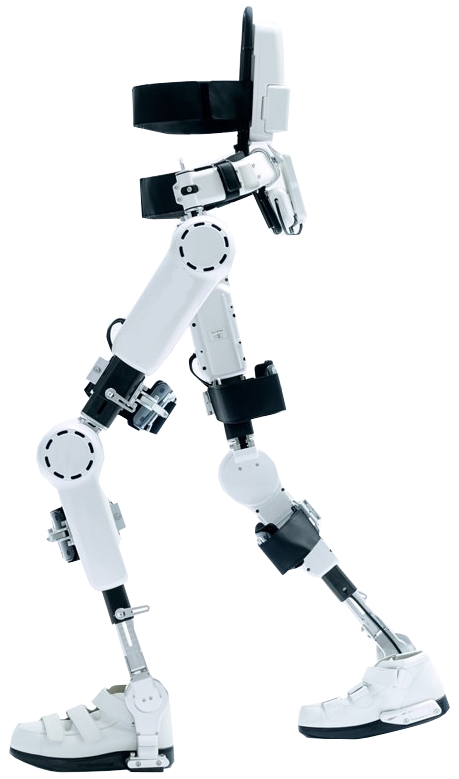
\includegraphics[width=.3\textwidth]{images/fig_01}}
\def\xxpied{%
Cycle 07 -- Modélisation des chaînes de solides \\%dans le but de déterminer les contraintes géométriques dans les mécanismes\\% afin de valider leurs performances.\\
Révisions 1 -- 2 -- 3 -- \xxactivite%
}

\def\xxposongletx{2}
\def\xxposonglettext{1.45}
\def\xxposonglety{20}
%\def\xxonglet{Part. 1 -- Ch. 3}
\def\xxonglet{\textsf{Cycle 01}}
